\part{Sleep Detection}

    \chapter{Overview}

        This section covers the development and evaluation of the sleep detection algorithm. The algorithm aims to extract features like sleep onset time, wakefulness onset time, and total time asleep from accelerometer data recorded on a wrist-mounted device.

        The basis of the algorithm relies on the fact that the level of activity of a person can be determined from the magnitude of the standard deviation or the energy of the accelerometer signal. If there is no movement, the standard deviation will simply be the square root of the variance of the noise in the accelerometer sensor data (assumed to be zero-mean Gaussian). If there is a high level of movement, then there will be a high standard deviation from the mean signal. If there is a long period of low activity then this period will be defined as corresponding to sleep time. This set of rules and inferences will be the guiding principles upon which the algorithm is built.


    \chapter{Database}
        \label{c-database}

        Algorithm development and testing described in this chapter relies on a database created by Borazio et al. at TU Darmstadt \cite{borazio}. The database contains accelerometer data from 42 patients, their clinically annotated polysomnography results, and light sensor data from overnight stays in a sleep lab. The patient undergoing polysomnography in a sleep lab has their electroencephalogram, oxygen levels in the blood, heart rate, breathing, eye movement, and leg movement recorded. A trained professional, then produces a report summarising the transitions between sleep stages (deep sleep, Rapid Eye Movement (REM), awake) during the night. The accelerometer data in the Darmstadt database comes from a custom device that is mounted on the wrist of the patient. The data is logged at 100Hz. The data collected by Borazio e. al. was collected from 42 sleeping lab patients aged between 28 and 86 years old. These patients were suffering from a variety of sleeping disorders, later diagnosed as primarily sleep apnea syndrome (SAS), restless leg syndrome (RLS), or narcolepsy. In total, 45 nights of data were collected, with three patients providing 2 nights' worth of data \cite{borazio}.

        The data provided is contained and compressed in such a way that it requires reformatting prior to the use in the algorithm described below. Each patient record has its own file (a .npy file, used for Numpy calculations in Python) which contains 7 columns: a timestamp, the runlength encoding, x-acceleration, y-acceleration, z-acceleration, light sensor value, and a ground truth value. The runlength encoding represents how many times in a row does the set of measurements that follows repeat, for example runlength encoding of $10$ represents 10 identical copies of the data (x,y,z acceleration, light sensor, and ground truth) with increasing timestamps. 

        All of the acceleration data is stored in 8-bit unsigned integer format, from 0 to 255. According to Borazio, et. al. this maps to an acceleration value of $-4g$ to $4g$, where $g$ is gravity. The light sensor value is not used in this project and as such will be disregarded. The ground truth data is coded as follows: 0 indicates unknown sleep state, 1-3 maps to different sleep states rated from deepest to lightest, 5 indicates random eye movement (REM) sleep, 6 indicates awake, and 7 indicates movement.

        In order to format this data to fit the needs of this project, a few steps were taken:

        \begin{itemize}
            \item The x,y, and z accelerations were linearly mapped back to $[-4g,4g]$ and the magnitude calculated as $\sqrt{x^2 + y^2 + z^2}$.
            \item The light sensor value was removed from the data.
            \item The runlength encoding was decoded.
            \item The data was downsampled to $10Hz$ to extend the battery life of the wearable device which will eventually be used in the application of this algorithm.
        \end{itemize}

        The downsampling is a simple operation: keep one point out of every 10 after the runtime encoding decoding is complete. Decoding the runlength encoding is equally simple: duplicate the row of $n$ times where $n$ is the runlength encoding for that row.

        \section{Acceleration Scaling}

            An original value of $127$ corresponds to $0g$ and thus the value of acceleration can be derived from:

            \begin{equation}
                a_n = (a_o - 127)*\frac{8*g}{256}
            \end{equation}
            where $a_n$ is the new acceleration value, $a_o$ is the original, integer value of acceleration, and $g=9.81\frac{m}{s^2}$ is gravity.

            This approach is validated by ensuring that the magnitude of the signal is always gravity or higher. This was true for the reformatted dataset, hence this approach is appropriate.



    \chapter{Sleep-Detection Algorithm Description}

        The algorithm works in two stages: the classification stage and the post-classification filter. The algorithm is designed to work with data sampled at 10Hz. 

        \section{Pre-Classification Filter}

            Originally, the design included a pre-classification filter. However, this was removed as it was found to degrade overall performance. The implementation and explanations for the removal of the filter are described below.

            The aim was to remove high-frequency noise and attenuate spikes from the signal. This was done with a simple moving average filter, with the following coefficients:

            \begin{equation}
                h_k = \frac{1}{N}, 1\leq k\leq N
            \end{equation}
            where $h_k$ is the $k^{th}$ coefficient of the filter and $N$ is the length of the filter.

            The frequency response of this filter can be seen below in Figure \ref{img_pp_filter}. Body movement during sleep is generally slow, so a filter removing higher frequency data is desired in this use case.

            \begin{figure}[h]
                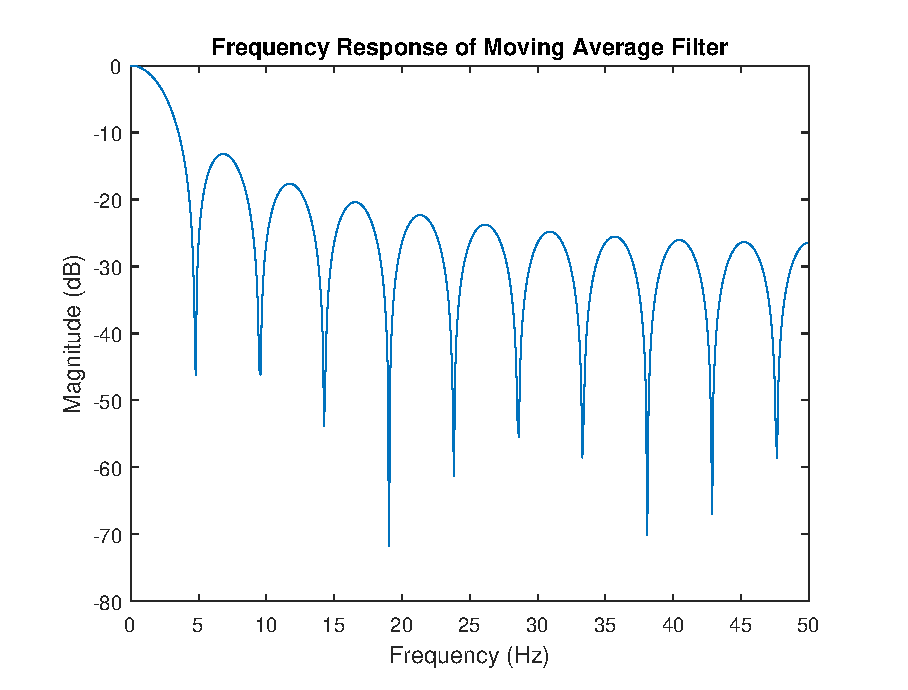
\includegraphics[width=\textwidth]{Images/sleep_pre_filter.eps}
                \centering
                \caption{Frequency response of the pre-classification filter with a length of 21 samples.}
                \label{img_pp_filter}
            \end{figure}

            An example of the data before filtering and after filtering can be seen below in Figure \ref{img_pp_filter_ex}.

            \begin{figure}[h]
                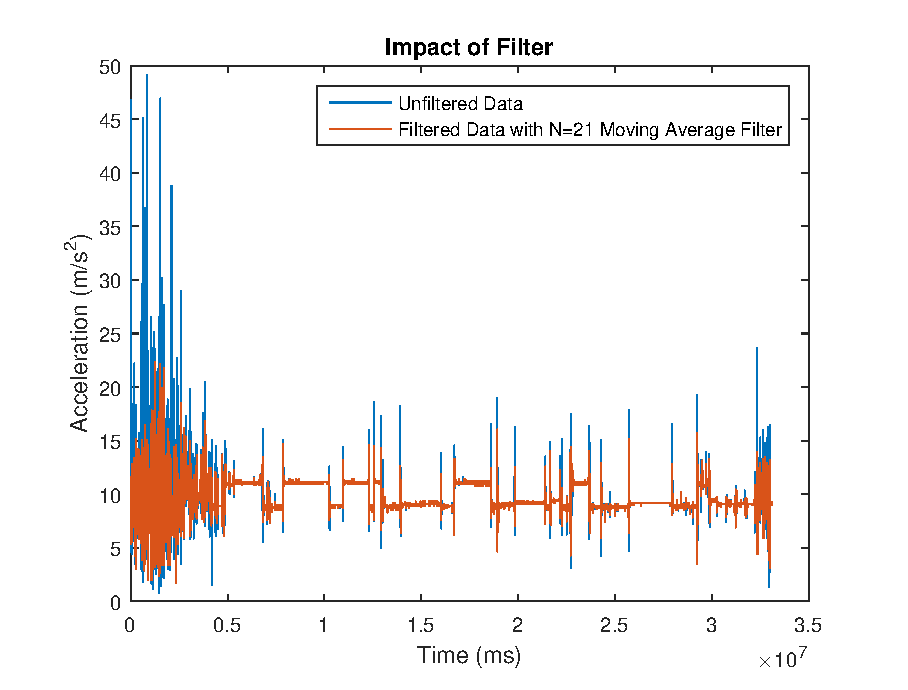
\includegraphics[width=\textwidth]{Images/sleep_pre_filter_ex.eps}
                \centering
                \caption{Example of data before and after filtering(blue before filter, orange after filter). Note the reduced magnitude in the active areas (areas of high magnitude.)}
                \label{img_pp_filter_ex}
            \end{figure} 

            This graph illustrates why the filter had to be removed. It decreases the amplitude of high-activity signals thus reducing the standard deviation. This has a direct impact on the parameter that we wish to estimate. Removing the filter increased the algorithm accuracy by around 5\%.           

        \section{Classification Stage}

            The next stage of the algorithm is to predict whether a segment of the signal corresponds to the subject being asleep or awake. The signal is divided into segments 300 samples long, equivalent to a period of 30 seconds at a 10Hz sampling frequency. This period was chosen as it is the segment length used in polysomnography, hence can be considered the minimum length of a sleep episode.

            \subsection{Data Characterization}

                There is only one variable upon which the classification is done, so a simple analysis can be done to obtain a threshold that will act as the decision boundary between the two classes: asleep and awake. The segments are separated based on their ground truth class (from polysomnography) and the mean and standard deviation are computed for each class. The probability density functions (pdf) can then be plotted. The decision boundary is the intersection of these two cruves. This can be seen in Figure \ref{img_pdfs}.

                \begin{figure}[h]
                    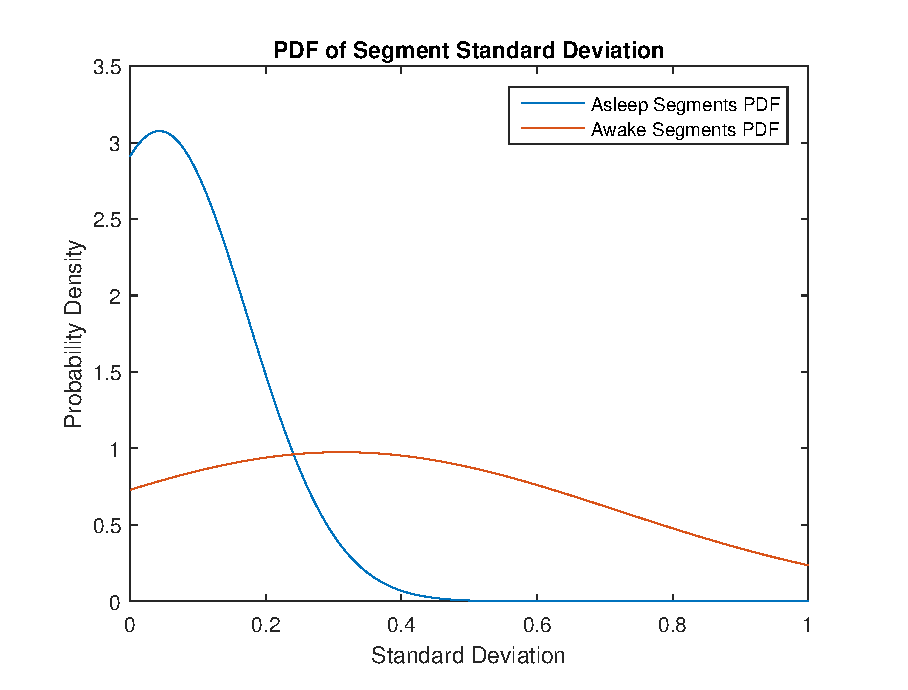
\includegraphics[width=\textwidth]{Images/segment_pdfs.eps}
                    \centering
                    \caption{The pdfs for both the asleep segments and awake segments. The intersection occurs at $\sigma = 0.221$.}
                    \label{img_pdfs}
                \end{figure}

            \subsection{Classification Process}

                Classification is performed through logistic regression. The weights of the regression are obtained through a learning process with the following steps:

                \begin{itemize}
                    \item Separate the segments into awake and asleep sets based on the ground-truth data from polysomnography.
                    \item To ensure a balanced training set (i.e. - equal number of each class) compute the number of segments for training through $n = \frac{min(l_{awake},l_{asleep})}{2}$ where $l_{set}$ is the length of the set.
                    \item Randomly select $n$ segments from each of the asleep and awake sets. Train on this data.
                    \item Test the learned coefficients on the remaining segments not used in training verify that the training data was not overfitted.
                \end{itemize}

                The logistic classifier is defined as:

                \begin{equation}
                    p(\mathbf{x}, \mathbf{m}) = \frac{1}{1 + e^{-\mathbf{mx}}}
                \end{equation}
                where $\mathbf{x}$ is the feature vector and $\mathbf{m}$ is the coefficient vector. If $p(\mathbf{x}) \geq 0.5$ then that point is classified as asleep (or 1). Otherwise is classified as awake (or 0).

                To allow for the possibility of including more than one feature, the algorithm was implemented using a feature vector. When there is only one feature (the standard deviation of the accelerometer data), the feature vector contains 2 elements: a constant (to serve as a bias), and the aforementioned standard deviation. This is defined as follows: 

                \begin{equation}
                    \mathbf{x} = \begin{bmatrix} 1 & \sigma \end{bmatrix}
                \end{equation}

                To train the classifier, a loss function needs to be minimized. To derive this, start with the likelihood of the coefficients given the data:

                \begin{equation}
                    \mathcal{L}(\mathbf{m}) = \prod_{i=1}^n p(y_i|\mathbf{x_i}, \mathbf{m})
                \end{equation}
                where $\mathcal{L}(m)$ is the likelihood of the coefficients, $y_i$ is the ground truth of the $i^th$ data point.

                If the log-likelihood is considered, then this expression can be expanded to:

                \begin{equation}
                    \log{\mathcal{L}(\mathbf{m})} = \sum_{i=1}^n (y_i\log{p(\mathbf{x_i}, \mathbf{m})} + (1-y_i)\log{(1 - p(\mathbf{x_i}, \mathbf{m}))})
                \end{equation}
                where the first term under the summation represents the contribution to the likelihood when $y_i = 1$ and the second term represents the contribution when $y_i = 0$.

                If the log-likelihood is differentiated with respect to $\mathbf{m}$ then it can be shown that the differential is given by:

                \begin{equation}
                    \frac{\partial}{\partial \mathbf{m}}\log{\mathcal{L}(\mathbf{m})} = \sum_{i=1}^n (y_ip(\mathbf{x_i}, \mathbf{m})\mathbf{x_i} - (1-y_i)(1 -p(\mathbf{x_i},\mathbf{m}))\mathbf{x_i})
                \end{equation}

                Unfortunately, this expression has no closed form solution if set to zero. Logistic regression can only be optimized using methods like gradient descent. The premise of gradient descent is simple: calculate the gradient at a point and then move either up or down the gradient, for maximization and minimization respectively. The downside of this method is that there is no guarantee of finding the global maximum, merely a local maximum. 

                In this project, the training and testing was performed by a Python package called scikit. The coefficients yielded are given by:

                \begin{equation}
                    \mathbf{m} = \begin{bmatrix} 0.8321 & -8.1804 \end{bmatrix}
                \end{equation}
                where the first coefficient is related to the constant and the second coefficient is related to the standard deviation. For the training dataset, the final accuracy with these coefficients was 72.9\% and for the testing dataset it was 71.2\% which shows the data was not overfitted during training.

                The decision boundary for the logisitic classifier is shown in Figure \ref{img_regression}. The boundary occurs at $\sigma = 0.11$.

                \begin{figure}[h]
                    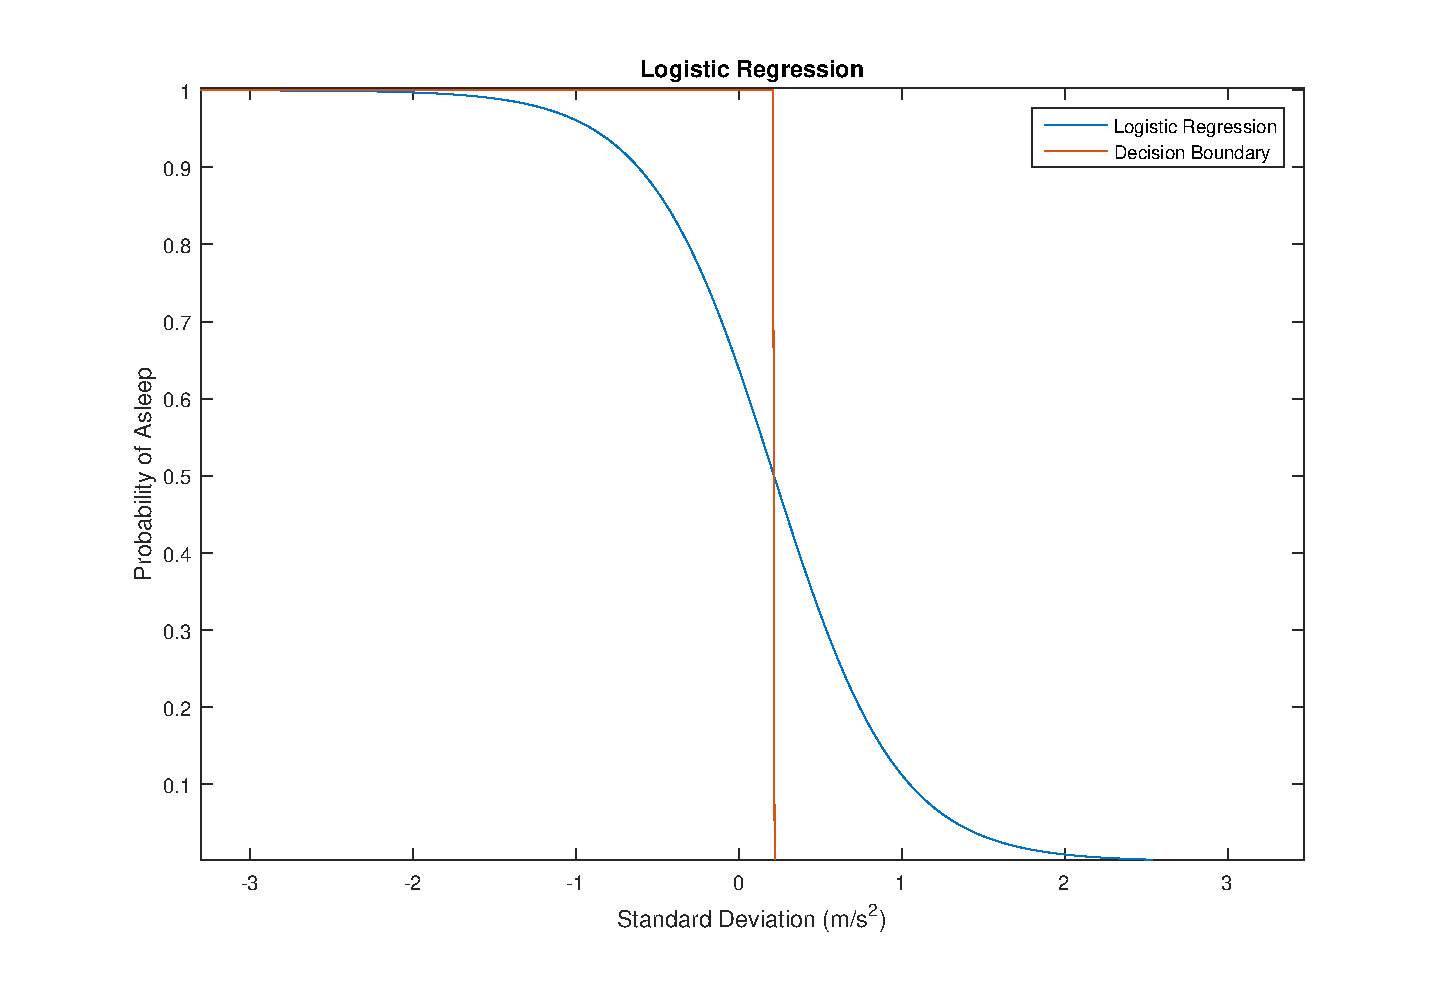
\includegraphics[width=0.75\textwidth]{Images/logistic_regression.eps}
                    \centering
                    \caption{A plot of the standard deviation of a signal segment against the probability of the subject being asleep. The step function represents the decision boundary based on $p(x) = 0.5$.}
                    \label{img_regression}
                \end{figure}

                An example of the classified data can be seen below in Figure \ref{img_regression_ex}. Recall that the output from the logistic regression provides the binary classification: if $p(x) > 0.5$ then the midpoint of the 30-second segment is assigned to class 1 (asleep), otherwise it is assigned to class 0 (awake).

                \begin{figure}[h]
                    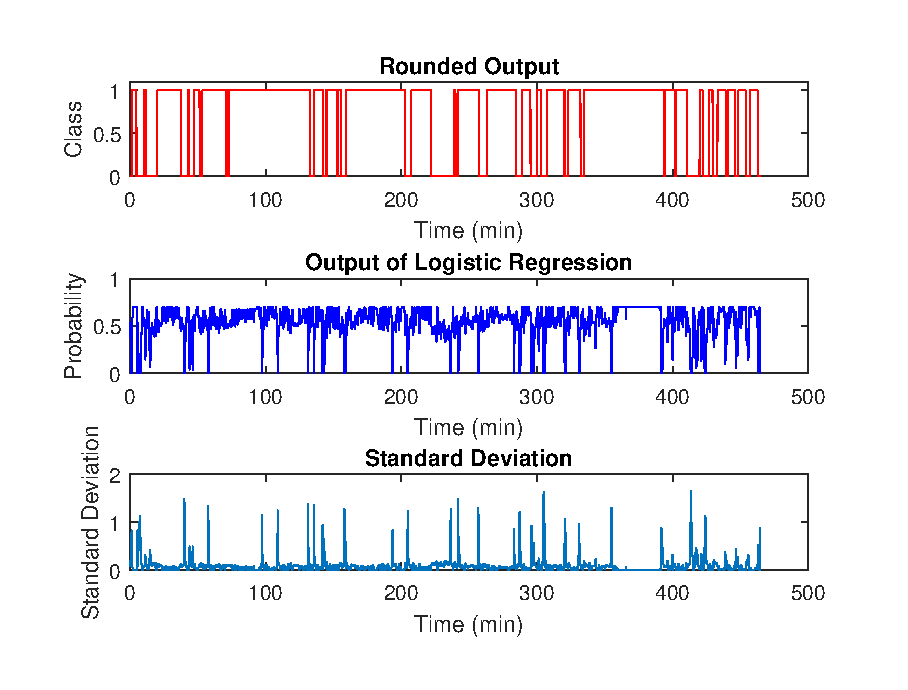
\includegraphics[width=0.8\textwidth]{Images/logistic_regression_ex.eps}
                    \centering
                    \caption{An example of the logistic regression classifying the data. From top to bottom: local standard deviation, logistic regression probability, and rounded output.}
                    \label{img_regression_ex}
                \end{figure}

        \section{Post-Prediction Filter}

            The next and final stage is a post-classification filter. It is reasonable to assume that for our purposes, the minimum sleep time detectable is approximately $5$ minutes. The filter works as a hard-limiter, that is to say, if the output of the filter is above some threshold, the output gets rounded up to 1.0 and all other values get rounded down. This is to maintain the 0-1 classification inherent in the problem. Note that this is an additional hard-limiter to the hard-limiter inherent in the logistic regression classifier.

            For any sample, a window is centered on that sample with $k$ points to the left and $k$ points to the right of this point. The filter value is calculated as follows:

            \begin{equation}
                f_n = \sum_{i=-k}^k h_ix_{n+i}
            \end{equation}
            where $f_n$ is the filter value at the $n^{th}$ point, $h_i$ is the $i^{th}$ filter coefficient and $x_{n+i}$ is the $(n+i)_{th}$ point. If $f_n$ exceeds $t$, a chosen threshold, then the $n^{th}$ point is marked as corresponding to asleep. $k$ is set to $1500$ for this filter, deriving from the $5$ minute minimum. 

            Two windows were considered for this filter: a moving average window (flat) and a Gaussian window. With the moving average window each point inside the window is valued equally such that $h_i = \frac{1}{2k + 1}$. With the Gaussian windows points closer to the point under consideration are weighted more heavily than those farther away such that $h_i = \frac{1}{\sqrt{2\pi \sigma_f}}e^{\frac{-(i-k)^2}{2\sigma_f^2}}$ where $\sigma_f$ is the standard deviation of the filter.

            The threshold, $t$ was varied for both filters from $0.5$ to $1$ in $0.1$ increments and the standard deviation, $\sigma$, for the Gaussian filter was varied from $1000$ to $3000$ in $500$ increments. After this coarse search was done, the optimization was repeated for thresholds around the maximum from the previous step in increments of $0.01$. The $\sigma$ values were chosen to align with the filter length of $3001$, ensuring that all values have a non-negligible weight, as filter coefficients at points outside of the $\begin{bmatrix}-2\sigma & 2\sigma \end{bmatrix}$ range are effectively given zero weighting.

            The best performing filter was the Gaussian with $t=0.580$ and $\sigma=2500$. An example of this post-classification filter in action is shown below in Figure \ref{img_post_filter_ex}.

            \begin{figure}[h]
                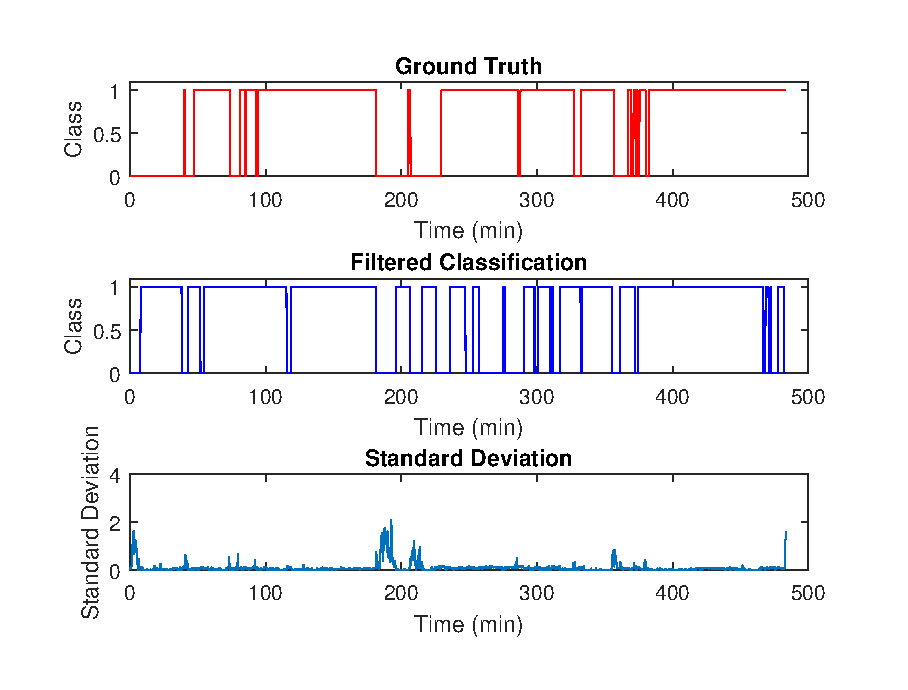
\includegraphics[width=0.8\textwidth]{Images/post_prediction_filters_ex.eps}
                \centering
                \caption{An example of the classified output being filtered. The filter used was a Gaussian filter with length 3001, standard deviation of 2500 and threshold 0.58. From top to bottom: local standard deviation, logistic regression probability, rounded output, filtered classification, and ground truth.}
                \label{img_post_filter_ex}
            \end{figure}


    \chapter{Results}

        The results presented here are the result of running the algorithm described above, with no pre-classification filter, over $45$ of the $46$ data records in the Darmstadt database. One of the records was rejected as there was very little sleep in the record and the data was inconsistent throughout.

        An example of the algorithm classification in action can be seen in Figure \ref{img_ex_data_recording}. Note that a state of 1 indicates sleep, a state of 0 indicates wakefulness. 

        \begin{figure}[h]
            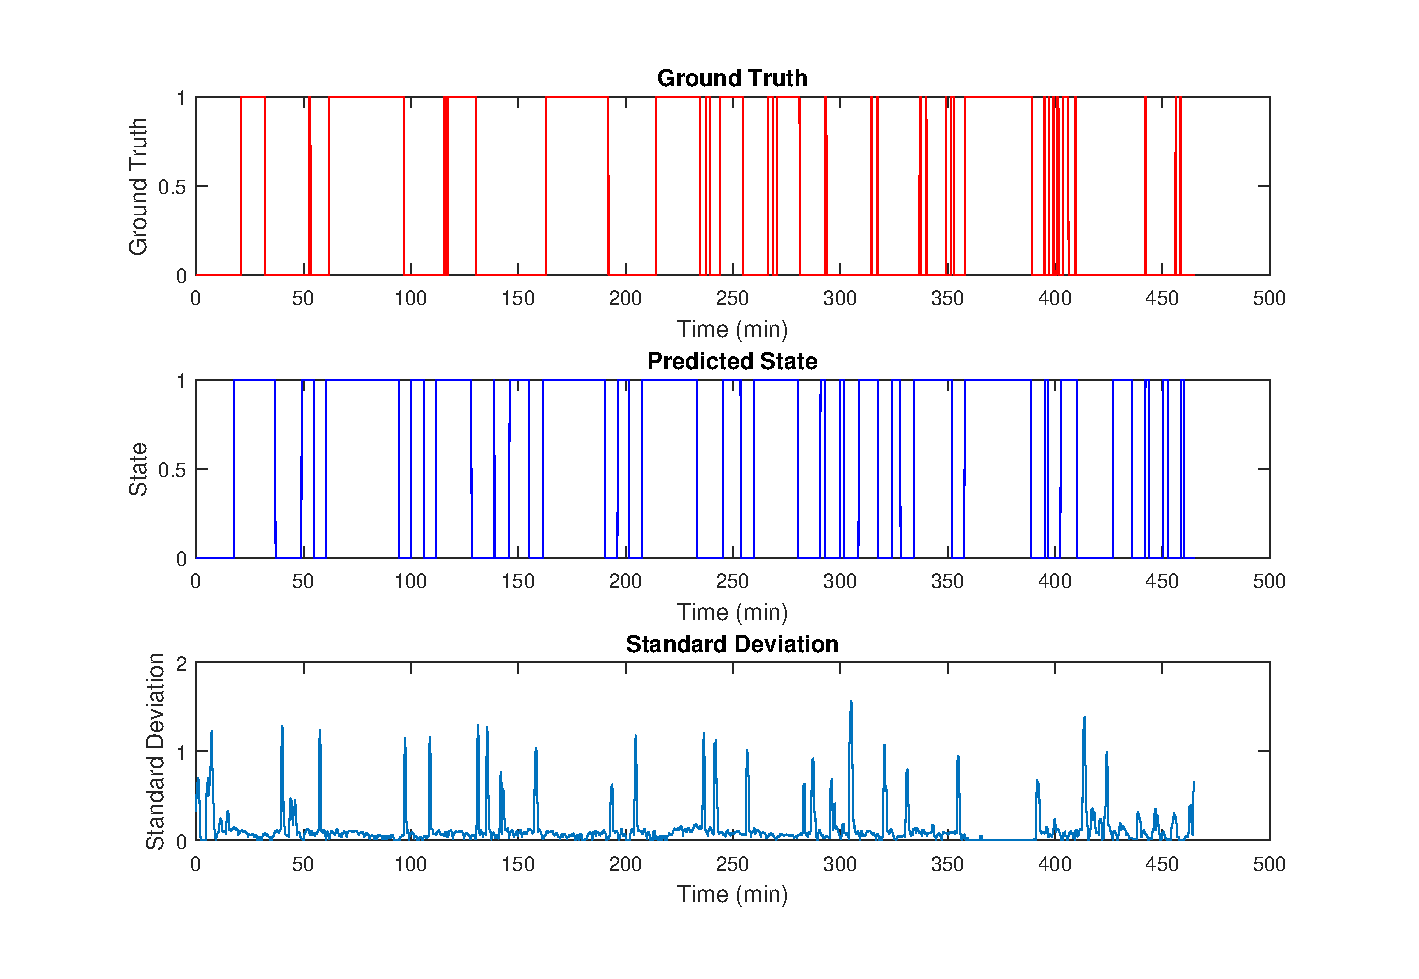
\includegraphics[width=\textwidth]{Images/example_data_recording.eps}
            \centering
            \caption{Example of the classification algorithm. From top to bottom: ground truth, classification output, standard deviation.}
            \label{img_ex_data_recording}
        \end{figure}

        \section{Statistics}

            The performance of the algorithm is assessed using 3 metrics: the Total Time Asleep (TTA), the total amount of sleeping time in the record, the Sleep Onset Time (SOT), the timestamp of the first incidence of sleep, and the Wakefulness Onset Time (WOT), the timestamp of the last incidence of sleep. The latter two parameters are representative of the start and end of a night's sleep. 

            For the algorithm described above, the following results are obtained.

            \begin{center}
                \captionof{table}{Results for the sleep detection algorithm.}
                \label{tbl_sleep_errors}
                \begin{tabular}{|c||c|c|}
                    \hline
                    Metric & Mean Error & Median Error \\
                    \hline
                    Total Time Asleep (\%) & 22.64\% & 10.93\% \\
                    Sleep Onset Time (minutes) & 25.35 min & 19.37 min \\
                    Wakefulness Onset Time (minutes) & 19.00 min & 8.48 min \\
                    \hline
                \end{tabular}
            \end{center}

            In comparison, the algorithm presented performs better than the algorithm described in Borazio, et. al. \cite{borazio} which achieved 21.17\% median error for Total Time Asleep (TTA). The paper from Borazio et al. makes no mention of Sleep Onset Time (SOT) or Wakefulness Onset Time (WOT) statistics, so there cannot be a comparison here.

            From the results, it is clear that all the error statistics have outliers far from the median since $e_{mean} > e_{median}$ for all the statistics. This is confirmed by the boxplots of the errors shown Figures \ref{img_tta_error} and \ref{img_sot_wot_error}. For example, for the boxplot of TTA there are a number of outliers that skew the mean away from the median, but the bulk of the errors is found between $5\%$ and $32\%$ error. 

            \begin{figure}[h]
                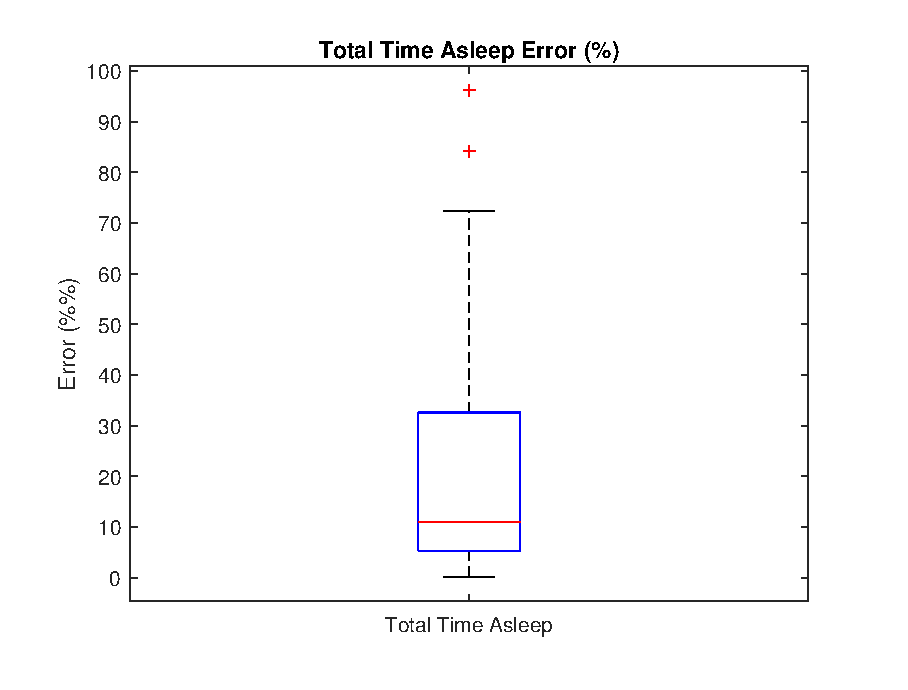
\includegraphics[width=0.75\textwidth]{Images/tta_error.eps}
                \centering
                \caption{Boxplot of errors for the Total Time Asleep. Median is at 11.89\%.}
                \label{img_tta_error}
            \end{figure}

            \begin{figure}[h]
                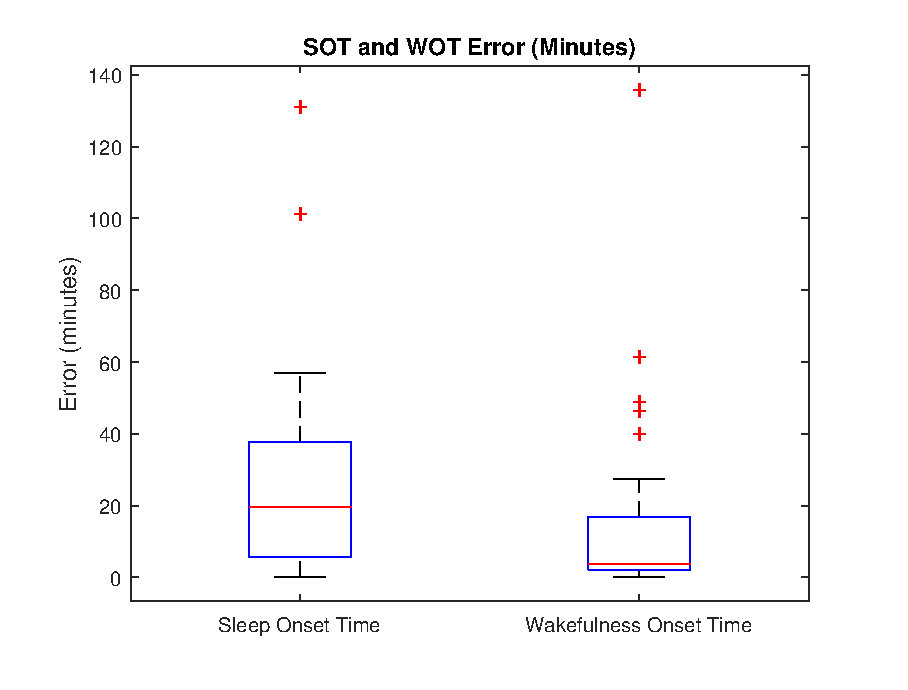
\includegraphics[width=0.75\textwidth]{Images/sot_wot_error.eps}
                \centering
                \caption{Boxplots of errors for the Sleep Onset Time and Wakefulness Onset Time. Note that the WOT is generally more accurate than the SOT.}
                \label{img_sot_wot_error}
            \end{figure}

            Another interesting phenomenon is the difference in accuracy between the SOT and WOT, as these fundamentally represent the two abilities of the algorithm: to identify sleep and wakefulness segments respectively. One explanation for the WOT being generally more accurate is that the end of sleep is usually close to the end of the recording. This limits the WOT error, whereas a similar phenomenon does not occur with the SOT.

        \section{Precision and Recall}

            Precision is defined as "the fraction of retrieved instances that are relevant" and recall is defined as "the fraction of relevant instances that are retrieved" \cite{prec_rec}. Here sleep precision is the percentage of classified sleep states that are sleep states in the ground-truth data. Sleep recall is the percentage of ground-truth sleep states that are classified as sleep states. The precision and recall were calculated on a per recording basis and tabulated for the entire database. The results of this can be seen in Figure \ref{img_prec_recall}.

            \begin{figure}[h]
                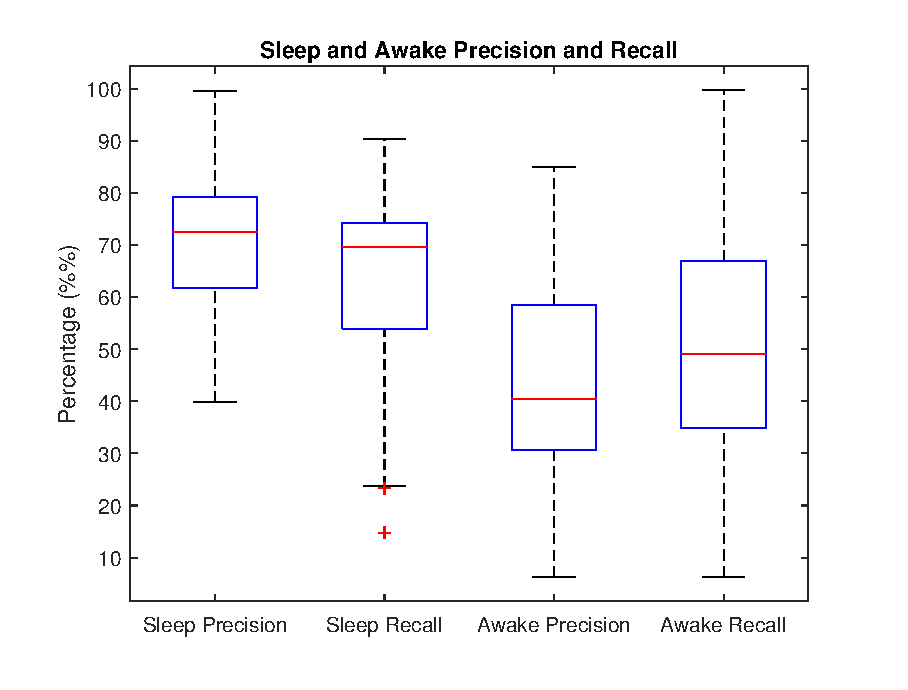
\includegraphics[width=0.75\textwidth]{Images/prec_recall.eps}
                \centering
                \caption{Boxplots of precision and recall for sleep and awake states. From left to right: sleep precision, sleep recall, awake precision, awake recall.}
                \label{img_prec_recall}
            \end{figure}

            The first point to note is that sleep precision is generally higher than awake precision. An explanation for this is that the algorithm is more biased towards classifying a sample as awake than sleep. This means that the algorithm will only classify a sample as corresponding to sleep when it is very sure about the state, that is to say the default assumption is that the sample corresponds to awake. Another point to note is that there is a very large variance in the awake precision and recall. This means that the algorithm generally has a hard time correctly identifying awake states. The awake recall being higher than precision indicates again that the algorithm has a default assumption that any given sample corresponds to awake. 

            In Borazio et al. the authors behaved the opposite way, along with the Cole \cite{cole} and Oakley \cite{oakley} algorithms, in that they tended to bias towards classifying a sample as belonging to the sleep state. This is evidenced by the awake recall being slightly higher in our algorithm (51\% median vs. 45\% for Borazio et al.). This however, comes at the cost of a reduced sleep recall (72\% vs 94\% for Borazio et al.).

            This presents an interesting trade-off that may be made when selecting the optimal algorithm. The algorithm developed in this project gives better performance with respect to the estimation of Total Time Asleep, whereas the recall statistics for the Borazio et al. were generally better. If the application of the algorithm was purely for recording the time spent asleep each night, as may be the case when tracking the well-being of a healthy individual, then the algorithm presented in this report would be the better choice. On the other hand, if the application was geared towards identifying and tracking sleep fragmentation during the night (which reflects the condition of an individual with a chronic disease such as COPD or heart failure), an algorithm that has generally better recall statistics, like those presented by Borazio et al., would be the better choice. 


    \chapter{Further Work}

        Although small improvements were made to the sleep detector, there is still room for significant improvement. One area that can be explored is extending the feature vector used for classification. Other features of the signal segment like the skewness or kurtosis of the distribution could be explored. The frequency content of the signal could also be investigated, in an attempt to correlate this with the sleep state. Ultimately, this approach is limited due to the simple fact that it is impossible to differentiate between the situation in which someone is awake and not moving and the situation in which someone is sleeping. 

        One other area of interest would be to explore extending the algorithm to include more sensors than the accelerometer, for example recording heart rate or light intensity, using these factors as additional features. The structure of the algorithm is designed to accommodate additional features as these can simply be added to the feature vector without otherwise changing the algorithm.